\section{Benchmarks}
I use two stencil kernels: a very simple one to test the water, and hypterm, a kernel from real Compressible Navier Stokes application.

\subsection{Simple Stencil}
Algorithm \ref{alg:simple} shows what the simple stencil computes. GPU algorithm will look slightly different since it will be instructions for each thread to work on just their assigned portion. Also, since stencil computation is bandwidth-bound, we have to be careful about reading data or the memory access time will dominate in most cases and that wouldn't be interesting to tune.
To make the most reuse of data, I followed NVIDIA's Micikevicius optimized approach \cite{nvidia_25p-stencil}. In essence, we create 2D thread blocks. Each thread $(i,j)$ will work on the points $x(f(i),g(j),:)$ (moving along the z direction). At the beginning, before computation, all threads in the same block coordinate on loading the plane $z=k_0$ into shared memory, then compute the stencil operation, sharing the data as illustrated in Figure \ref{fig:25-point_stencil}. Then the threads moves on to next $z=k_0+1$ altogether and coordinating on loading plan $z=k_0+1$ and so on. This way all threads can share most of the data in the xy plane and only have to pay for the data they loads in the z direction. However, this is not expensive either, since 7 of the 8 values it read in the first step is reused in the next step, and thus it only needs to load one more new value for the z direction. The full algorithm is listed in Algorithm \ref{alg:simple-gpu}. Both this and the hypterm kernel use double-precision floating-point.

\begin{algorithm}
\floatname{algorithm}{Algorithm}
\caption{\textsc{Simple Stencil on CPU}}
\label{alg:simple}
\begin{algorithmic}[1]
\State \emph{Input/Output:} $x$
\State \emph{Define $\phi_x(x,i,j,k)$:} Linear combination of $x[i-4:i+4,j,k]$
\State \emph{Define $\phi_y(x,i,j,k)$:} Linear combination of $x[i,j-4:j+4,k]$
\State \emph{Define $\phi_z(x,i,j,k)$:} Linear combination of $x[i,j,k-4:k+4]$
\For{each \emph{coordinate (i,j,k)} in $grid$}
	\State $x[i,j,k] \leftarrow -\phi_x(x,i,j,k) - \phi_y(x,i,j,k) - \phi_z(x,i,j,k)$
\EndFor
\end{algorithmic}
\end{algorithm}
\begin{algorithm}
\floatname{algorithm}{Algorithm}
\caption{\textsc{Simple Stencil on GPU (For Each Thread)}}
\label{alg:simple-gpu}
\begin{algorithmic}[1]
\State \emph{Input/Output:} $x$
\State \emph{Define $\phi_x(x,i,j,k)$, $\phi_y(x,i,j,k)$, $\phi_z(x,i,j,k)$:} As in Algorithm \ref{alg:simple}
\State $[i,j,k] \leftarrow get\_my\_coordinate()$
\For{$z_{offset}$ = 1 to $thread\_z$}
	\State Coordinate with other threads in my block to load the plane $z=k+z_{offset}$
	\State $x[i,j,k+z_{offset}] \leftarrow -\phi_x(x,i,j,k+z_{offset}) - \phi_y(x,i,j,k+z_{offset}) - \phi_z(x,i,j,k+z_{offset})$
\EndFor
\end{algorithmic}
\end{algorithm}
\begin{figure*}[!t]
\centering
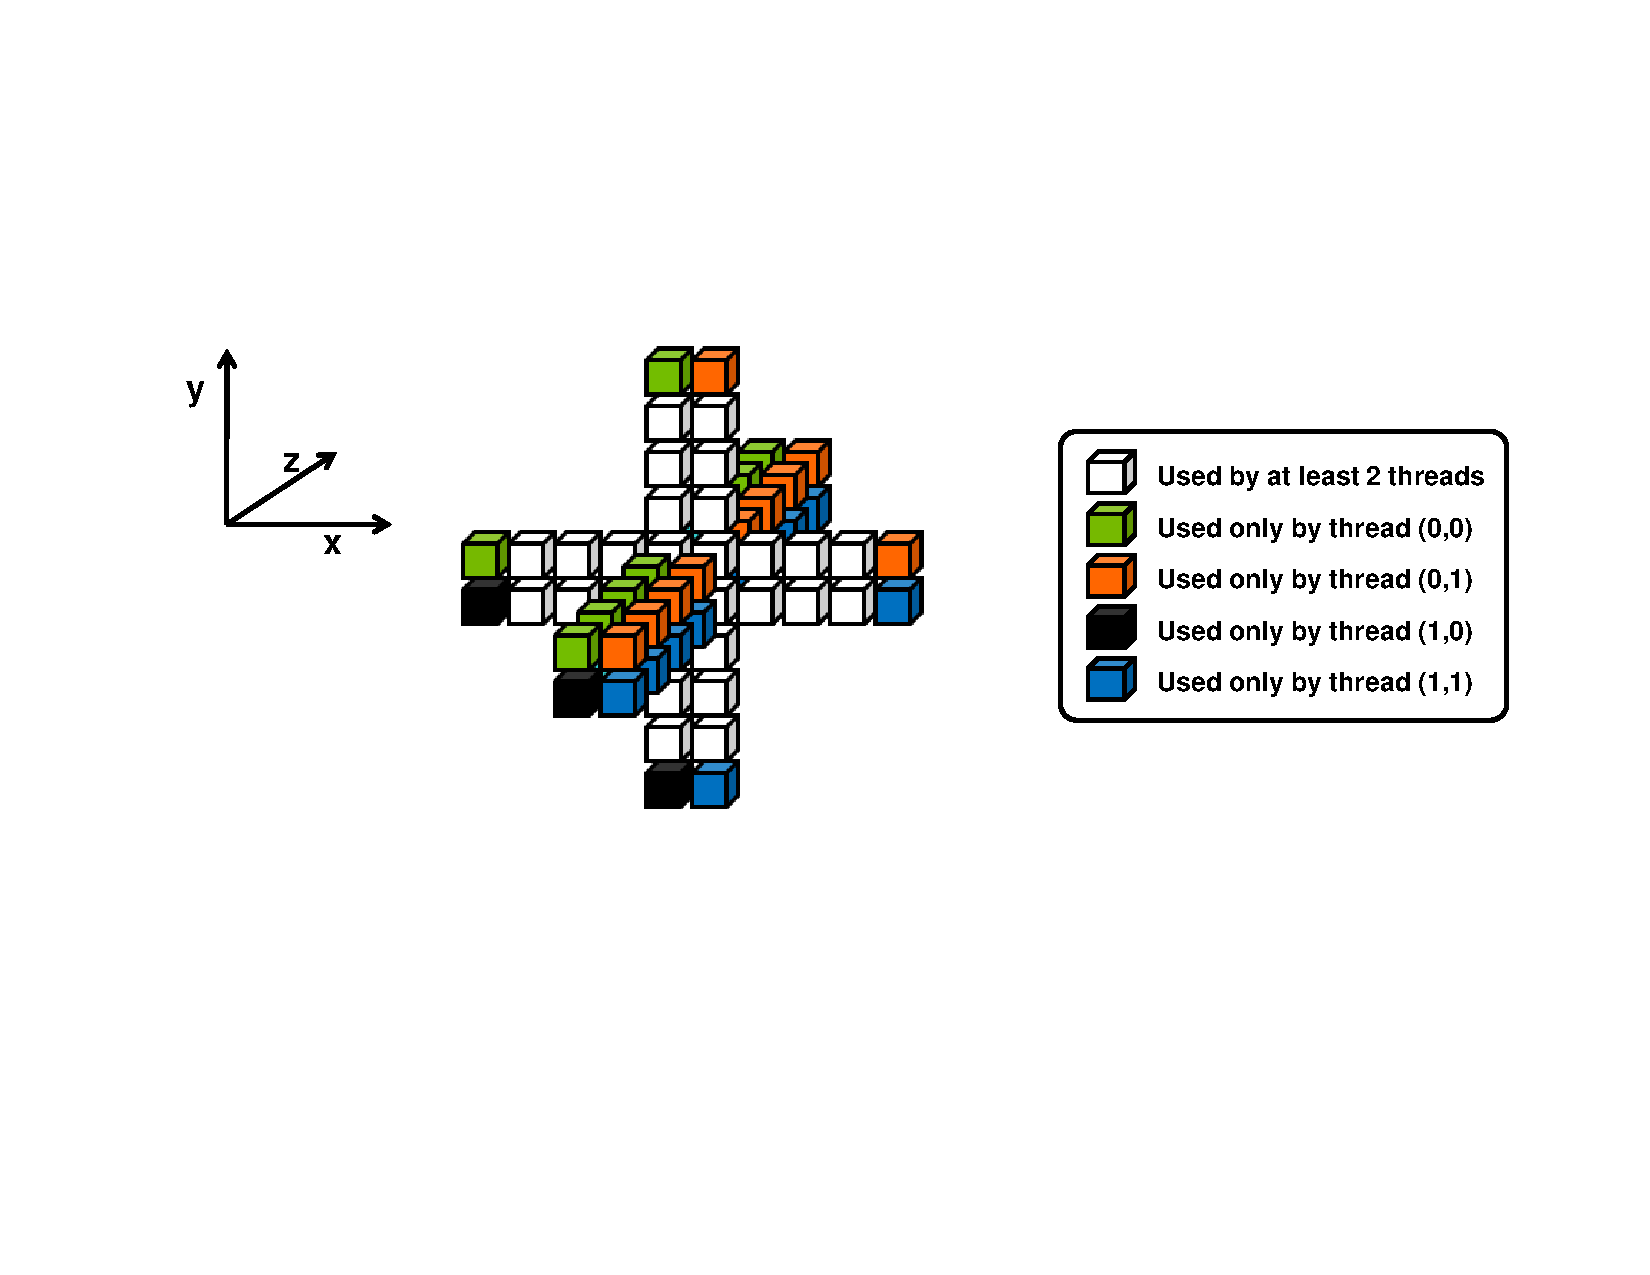
\includegraphics[width=0.8\textwidth]{./images/stencil-shared.pdf}
\caption{Illustration of Algorithm \ref{alg:simple-gpu}. (Courtesy of NVIDIA)}
\label{fig:25-point_stencil}
\end{figure*}

\subsubsection{Tuning Parameters}
As mentioned earlier, one of the most important parameters are thread block dimensions. CUDA supports up to 3 dimensions but since our algorithm uses 2D thread block we only have 2 variables $block\_dim\_x$ and $block\_dim\_y$. Next natural tuning parameter should also be obvious from the algorithm description. It is the number of points each thread process along the z dimension. I denote this with a variable $thread\_z$. The rest parameters are the limit on number of register a CUDA kernel can have ($maxrregcount$), the padding applied to shared memory ($shared\_pad$), the amount of available shared memory ($shared\_mem$), and whether if the kernel should bypass L1 cache ($bypass\_L1$), since its cache line is 128-bit wide and can sometimes hurt the performance. All the parameters are listed below.
% L1 supports reading 128-bit-aligned only

\begin{table}[h]
\center
\begin{tabular}{r c l}
$block\_dim\_x$ & $\in$ & $\{4, 8, 16, 32, 64, 128,256\}$	\\
$block\_dim\_y$ & $\in$ & $\{4, 8, 16, 32, 64, 128,256\}$	\\
$thread\_z$     & $\in$ & $\{4, 8, 16, 32, 64\}$			\\
$maxrregcount$  & $\in$ & $\{16, 20, 24, 28, 32\}$			\\
$shared\_pad$   & $\in$ & $\{32, 128, 256\}$				\\
$shared\_mem$   & $\in$ & $\{16, 48\}$						\\
$bypass\_L1$    & $\in$ & $\{0, 1\}$						\\
\end{tabular}
\end{table}

Counting normally, this would be a total of $7*7*5*5*3*2*2=14,700$ configurations. But the search space is actually a lot smaller, since some configurations are not feasible or valid on GPU. Pruning with GPU constraints, we are left with 7,350 configurations.

\subsection{Hypterm Kernel}
Hypterm is a kernel that computes hyperbolic terms in Compressible Navier Stokes application. It simply consists of many stencil computations as shown in Algorithm \ref{alg:hypterm}
\begin{algorithm}
\floatname{algorithm}{Algorithm}
\caption{\textsc{Hypterm}}
\label{alg:hypterm}
\begin{algorithmic}[1]
\State \emph{Input:} $q_x, q_y, q_z, q_{pres}, u_{imx}, u_{imy}, u_{imz}, u_{iene}$
\State \emph{Output:} $flux_{irho}, flux_{imx}, flux_{imy}, flux_{imz}, flux_{iene}$
\State \emph{Define $\phi_x(x,i,j,k)$, $\phi_y(x,i,j,k)$, $\phi_z(x,i,j,k)$:} As in Algorithm \ref{alg:simple}
\State \emph{Define $\psi_x(x,y,i,j,k)$:} Linear combination of $x[i-4:i+4,j,k]$ and $y[i-4:i+4,j,k]$
\State \emph{Define $\psi_y(x,y,i,j,k)$:} Linear combination of $x[i,j-4:j+4,k]$ and $y[i,j-4:j+4,k]$
\State \emph{Define $\psi_z(x,y,i,j,k)$:} Linear combination of $x[i,j,k-4:k+4]$ and $y[i,j,k-4:k+4]$
\For{each \emph{coordinate (i,j,k)} in $grid$}
	\State $flux_{irho}[i,j,k] \leftarrow -\phi_x(u_{imx},i,j,k) - \phi_y(u_{imy},i,j,k) - \phi_z(u_{imz},i,j,k)$
	\State $flux_{imx}[i,j,k] \leftarrow -\psi_x(u_{imx}.*q_x,q_{pres}, i,j,k) - \phi_y(u_{imy}.*q_y,i,j,k) - \phi_z(u_{imz}.*q_z,i,j,k)$
	\State $flux_{imy}[i,j,k] \leftarrow -\phi_x(u_{imx}.*q_x,i,j,k) - \psi_y(u_{imy}.*q_y,q_{pres},i,j,k) - \phi_z(u_{imz}.*q_z,i,j,k)$
	\State $flux_{imz}[i,j,k] \leftarrow -\phi_x(u_{imx}.*q_x,i,j,k) - \phi_y(u_{imy}.*q_y,i,j,k) - \psi_z(u_{imz}.*q_z,q_{pres},i,j,k)$
	\State $flux_{iene}[i,j,k] \leftarrow -\psi_x(u_{iene}.*q_x,q_{pres}.*q_x,i,j,k) - \psi_y(u_{iene}.*q_y,q_{pres}.*q_y,i,j,k) - \psi_z(u_{iene}.*q_z,q_{pres}.*q_z,i,j,k)$
\EndFor
\end{algorithmic}
\end{algorithm}

However, implementing it is not as easy as it seems, since GPU has limited memory (the limiting factor here is number of registers and shared memory). Having to keep track of this many data all at once, coupling with the fact that we need 24 points for each data and that we store results in double precision made the kernel completely different from the simple one. The performance would be harder to predict because the large amount of shared memory, and also register usage limits concurrency.

\subsubsection{Tuning Parameters}
The parameters are the same as the simple stencil kernel, with a slight changes in some set of parameter values to suit more with the Hypterm kernel. These create total of 6,931 valid configurations (pruned).
\begin{table}[h]
\center
\begin{tabular}{r c l}
$block\_dim\_x$ & $\in$ & $\{4, 8, 16, 32, 64, 128, 256\}$	\\
$block\_dim\_y$ & $\in$ & $\{4, 8, 16, 20, 24, 32, 40, 64, 80, 96, 128, 256\}$	\\
$thread\_z$     & $\in$ & $\{4, 8, 16, 32, 64\}$			\\
$maxrregcount$  & $\in$ & $\{32, 40, 48, 52, 64\}$			\\
$shared\_pad$   & $\in$ & $\{32, 128, 256\}$				\\
$shared\_mem$   & $\in$ & $\{16, 48\}$						\\
$bypass\_L1$    & $\in$ & $\{0, 1\}$						\\
\end{tabular}
\end{table}


